\documentclass{article}

\usepackage{polski}
\usepackage[utf8]{inputenc}
\usepackage{listings}
\usepackage{caption}
\usepackage{color}
\usepackage{graphicx}
\usepackage{hyperref}

\definecolor{dkgreen}{rgb}{0,0.6,0}
\definecolor{gray}{rgb}{0.5,0.5,0.5}
\definecolor{mauve}{rgb}{0.58,0,0.82}

\lstset{frame=tb,
  language=Python,
  aboveskip=3mm,
  belowskip=3mm,
  showstringspaces=false,
  columns=flexible,
  basicstyle={\small\ttfamily},
  numbers=none,
  captionpos=t,
  numberstyle=\tiny\color{gray},
  keywordstyle=\color{blue},
  commentstyle=\color{dkgreen},
  stringstyle=\color{mauve},
  breaklines=true,
  breakatwhitespace=true,
  tabsize=3
}

\DeclareCaptionFormat{listing}{#1#2#3}
\captionsetup[lstlisting]{format=listing,singlelinecheck=false, margin=0pt}



\title{Factorer MPI - dokumentacja projektowa}

\date{2016-06-07}

\author{Rafał Duraj, Piotr Dowgiałło, Bartosz Janusz, Maciej Kolański}

\begin{document}

%generowanie strony tytułowej
\pagenumbering{gobble}
\maketitle
\newpage  
\pagenumbering{arabic}

%spis treści
\tableofcontents
\newpage

\section{Temat projektu}

\paragraph{}W dzisiejszych czasach, gdy właściwie wszystko co robimy w jakiś sposób połączone jest z Internetem bezpieczeństwo jest bardzo ważnym tematem.

Faktoryzacja jest to proces podczas którego dla zadanego obiektu odnajduje się inne obiekty, które spełniają to, że ich iloczyn równy jest oryginalnemu obiektowi, w związku z czym te znalezione czynniki są w pewnym sensie od niego prostsze.

Podstawowy algorytm faktoryzacji bazuje na próbowaniu podziału liczby do faktoryzacji n przez wszystkie liczby pierwsze od 2 do $\sqrt{n}$. Tego typu algorytm bardzo dobrze radzi sobie z początkiem faktoryzacji liczby, bo dowolna liczba ma czynnik zarówno małe jak i duże. Jak wiadomo połowa wszystkich liczb dzieli się przez dwa, jedna trzecia licz przez trzy i tak dalej, a więc z dużym prawdopodobieństwem można pozbyć się w prosty sposób niskich czynników.

RSA jest to jeden z pierwszych i też obecnie najpopularniejszych asymetrycznych algorytmów kryptograficznych gdzie klucz jest publiczny. Bezpieczeństwo szyfrowania przy pomocy tego algorytmu jest związane z trudnością faktoryzacji dużych liczb.

\section{Zakres projektu}
\subsection{Cel}

\paragraph{}Celem projektu jest umożliwienie zlecenia zadania faktoryzacji dużej liczby (większych od $2^{64} -1$). Jednym z głównych założeń jest udostępnienie prostego w obsłudze interfejsu użytkownika i zmaksymalizowanie elastyczności – system powinień być zdolny do współpracy z zadanymi komputerami, a instalacja wymaganego oprogramowania musi być prosta. 

\subsection{Funkcjonalność}

\paragraph{Podstawowa}
\begin{enumerate}
	\item Udostępnienie mechanizmów rejestracji i logowania (konta użytkowników)
	\item Zarządzanie zadaniami z poziomu interfejsu webowego
	\begin{enumerate}
		\item zlecanie zadań
		\item przegląd historii
	\end{enumerate}
	\item Możliwość rozbudowy klastra bez ingerencji w kod
	\item Faktoryzacja metodą „brutalnej siły”
	\item Faktoryzacja metodą CFRAC
	\item Zachowywanie wyników pomyślanie wykonanych faktoryzacji
\end{enumerate}

\paragraph{Rozszerzona}
\begin{enumerate}
    \item Łamanie szyfru RSA
    \item Faktoryzacja metodą sita kwadratowego
    \item Forma graficznej prezentacji wyników pomiarów
\end{enumerate}

\section{Narzędzia i technologie zastosowane w projekcie}
\subsection{Zastosowane technologie}

\begin{figure}[h]
    \centering
    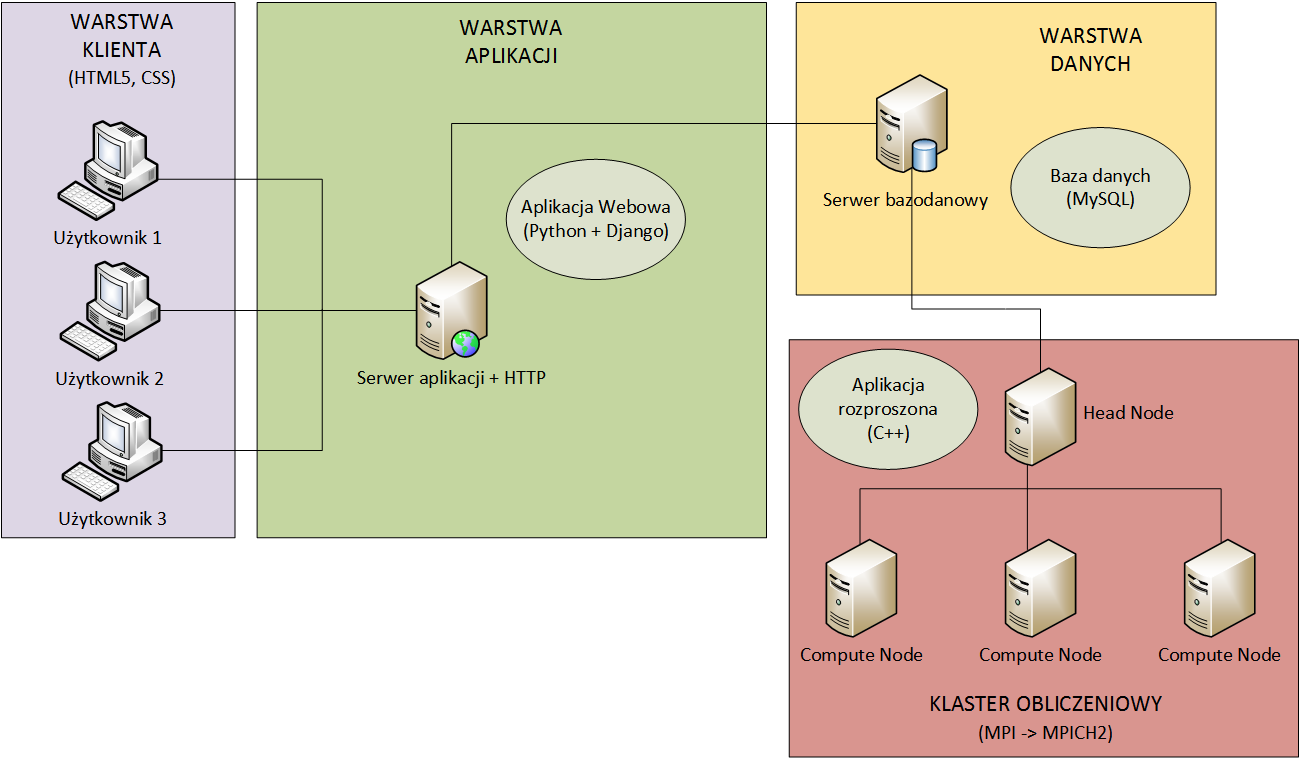
\includegraphics[width=1.0\textwidth]{schemat_blokowy_systemu.png}
    \caption{Schemat blokowy systemu}
    \label{fig:schemat}
\end{figure}

\paragraph{Strona klienta - HTML5, CSS}
Interfejs z którego bedzie korzystal klient projektowanego systemu został napisany w jezyku skryptowym HTML5 z użyciem stylów CSS. HTML5 jest obecnie standardem przy tworzeniu stron internetowych i w wiekszosci wyparl HTML4, w którego specyfikacji bylo duzo niescislosci. Uzycie CSS z kolei pozwoli ujednolicic prezentacje zawartosci w różnych przegladarkach, oraz uprosci organizacje samego kodu.

\paragraph{Aplikacja Webowa - Python 3.4 + Django 1.8.7\cite{django}}
Python jest jezykiem wysokiego poziomu ogólnego przeznaczenia, z kolei Django to framework webowy dla tego jezyka. Wybralismy ten zestaw z powodu wielu ulatwień przy tworzeniu aplikacji webowych, które sa przezeń oferowane, np. dynamiczny interfejs bazy danych, automatyczny interfejst administracyjny. Dodatkowo czesc naszej grupy jest zaznajomiona z tymi technologiami, wiec nie ma potrzeby poznawania ich od zera. Istotne sa tutaj wersje srodowisk - najnowsze dystrybucje nie obsluguja MySQL, w zwiazku z tym wybralismy poprzednie.

\paragraph{Baza danych - MySQL}
SZBD rozwijany przez firme Oracle. Charakteryzuje sie wszystkimi najwazniejszymi funkcjonalnosciami bazy danych oraz prostota tworzenia takiej bazy. Rozważalismy zastosowanie systemu Oracle Database, jednakże jest on zbyt rozbudowany jak na nasze potrzeby, a co za tym idzie trudny w obsudze. Mamy również doswiadczenie w integracji bazy MySQL z aplikacjami napisanymi w Pythonie (Django).

\paragraph{Klaster obliczeniowy - standard MPI\cite{mpich2}} MPICH2 to darmowa implementacja standardu MPI dla systemów Linux. Umożliwa proste tworzenie klastrów obliczeniowych, rozdzielania zadań miedzy poszczególne wezly i zbierania wyników. Oferuje interfejs dla jezyka C++. Jest wykorzystywany w wiekszosci topowych urzadzen wieloprocesorowych i ta popularnosc znaczaco wplynelo na jego wybór.

\paragraph{Aplikacaja rozproszona - C++11}
Wybór padl na ten jezyk ze wzgledu na jego znajomosc przez czlonków grupy oraz interfejs udostepniany przez srodowisko MPICH2.

\subsection{Narzedzia wykorzystane w projekcie}
\begin{itemize}
\item Aplikacja webowa PyCharm 5.0.4 - IDE do Pythona, obsuguje Django
\item Aplikacja rozproszona - CodeLite 9.1 IDE do C++, wersja na system Linux
\item Baza danych - developer do MySQL
\item Organizacja pracy - Trello (\url{https://trello.com/})
\item Hosting plików - GitHub (\url{https://github.com/}) 
\end{itemize}

\section{Aktualny stan rynku}

\paragraph{GGNFS (GPL'd implementation of General Number Field Sieve)} Aktywny rozwój. faktoryzacja liczb do 180 znaków, srednio do 140. Kilka wiekszych liczb tez. W wiekszosci przypadkow program GGNFS jest stabilny dla liczb skladajacych sie do 150-160 znakow. Posiada bugi. Nie jest czarna skrzynka, trzeba miec odpowiednia wiedze zeby go uzywać.

\paragraph{Cunningham Project} Projekt faktoryzujacy liczby $b^n +-1$ dla b=2,3,5,6,7,10,11,12 i duze n.\cite{cun}

\paragraph{RSA Factoring Challenge} Zawody zorganizowane przez RSA Security. Otwarte zawody dla wszystkich mające na celu zwiększyć zainteresowanie faktoryzacją liczb. Opublikowana została lista pseudopierwszych liczb (rozkładających się na dokładnie dwa czynniki), nazwanych liczbami RSA.Za rozłożenie niektórych z nich wyznaczono pieniężną nagrodę. Najmniejsza z nich, 100-cyfrowa liczba RSA-100 została rozłożona w ciągu kilku dni, ale większość do dziś pozostaje niezłamana.Zawody miały na celu śledzenie rozwoju możliwości komputerów w faktoryzacji. Jest to niezwykle istotne przy wyborze długości klucza w szyfrowaniu asymetrycznym metodą RSA. Postęp w łamaniu kolejnych liczb powinien zdradzać jakie długości klucza można jeszcze uznawać za bezpieczne.\cite{rsafactoringchallenge}

%Poczatkowo rekordy były bite za pomoca algorytmu CFRAC, który ustapił dopiero w latach 8XX w. algorytmowi sita kwadratowego. Za pomoca algorytmu QS sfaktoryzowano, miedzy innymi,liczby RSA-100, RSA-110, RSA-120 i RSA-129 [5]. Nast˛epnie na scen˛e wkroczył algorytm sita ciałliczbowego, który do dzis pozostaje najszybszym ze znanych algorytmów faktoryzacji i dzier ´ zy rekordy - najpierw RSA-640 (640 bitów, 193 cyfry) i RSA-200 (200 cyfr) w 2005 roku, a nast˛epnie RSA-768(232 cyfry) w 2009 roku, co pozostaje niepobitym rekordem do dzis.

%praca mgr Mateusz Niezabitkowski http://ki.agh.edu.pl/sites/default/files/usefiles/172/theses/mateusz.niezabitowski.algorytmy.faktoryzacji.w.zastosowaniach.kryptograficznych.v1.0-final.pdf

%Implementacje (eng wiki) : Some implementations focus on a certain smaller class of numbers. These are known as special number field sieve techniques, such as used in the Cunningham project. A project called NFSNET ran from 2002[6] through at least 2007. It used volunteer distributed computing on the Internet.[7] Paul Leyland of the United Kingdom and Richard Wackerbarth of Texas were involved.[8]

%Until 2007, the gold-standard implementation was a suite of software developed and distributed by CWI in the Netherlands, which was available only under a relatively restrictive license. In 2007, Jason Papadopoulos developed a faster implementation of final processing as part of msieve, which is in the public domain. Both implementations feature the ability to be distributed among several nodes in a cluster with a sufficiently fast interconnect.

%Polynomial selection is normally performed by GPL software written by Kleinjung, or by msieve, and lattice sieving by GPL software written by Franke and Kleinjung; these are distributed in GGNFS.

%NFS@Home GGNFS pGNFS factor by gnfs CADO-NFS msieve, which contains excellent final-processing code, a good implementation of the polynomial selection which is very good for smaller numbers, and an implementation of the line sieve. kmGNFS

%ElvenSmooth - projekt (... jeszcze nie doczytalem o nim dokladnie) http://home.earthlink.net/~elevensmooth/

%Factorizations of Cyclotomic Numbers http://www.asahi-net.or.jp/~KC2H-MSM/cn/

\section{Projekt techniczny}

\subsection{Klaster obliczeniowy}

\paragraph{Komunikacja}

\paragraph{Algorytm Brute Force}

\paragraph{Algorytm CFRAC}

\subsection{Strona internetowa}

\section{Dokumentacja powykonawcza (instalacyjna)}

\section{Istotne elementy kodu z komentarzem}

\section{Przykładowe wyniki badań efektywności programu równeległego}

\section{Wnioski}

\newpage
\begin{thebibliography}{9}
\bibitem{django}
	\emph{Dokumentacja Django}.
	\url{https://docs.djangoproject.com/en/1.8/},
	2016

\bibitem{mpich2}
	\emph{Dokumentacja MPICH2}.
  	\url{http://www.mpich.org/documentation/guides/},
  	2016.

\bibitem{cun}
	\emph{Cunningham Project}.
	\url{http://homes.cerias.purdue.edu/~ssw/cun/}

\bibitem{rsafactoringchallenge}
	\emph{RSA Factoring Challenge}.
	\url{http://pl.wikipedia.org/wiki/RSA_Factoring_Challenge}

\end{thebibliography}

\end{document}